\chapter{Cascade de Transducteurs}
\label{chap-cassys}

Ce chapitre presente l'outil \textit{Cassys} qui donne la possibilité de créer une cascade
de  transducteurs et de nouvelles manières de travailler sur la langue naturelle avec des 
graphes à états finis. Une \textit{cascade de transducteurs} \index{cascade de transducteurs}
applique plusieurs graphes (automates ou transducteurs), l'un après l'autre, sur le texte: chaque
graphe modifie le texte, et les changements peuvent être utilisés pour des traitements supplémentaires
par les graphes suivants. Ce type de  système est notamment utilisé pour l'analyse syntaxique, le chunking,
l'extraction d'information, la reconnaissance d'entitiés nommées etc. Pour faire cela, CasSys utilise
une succession de "locate patterns" avec les options adéquates.

\bigskip
\noindent Le premier prototype du système \textit{CasSys} \index{CasSys}  a été créé en 2002 au 
laboratoire LI (Laboratoire d'Informatique de l'Université de Tours) (\cite{these-nathalie}). 
Ce prototype était entièrement spécialisé pour l'extraction d'entités nommées. CasSys a été  
ensuite généralisé pour effectuer n'importe quelle sorte de traitement nécessitant une cascade. 
Il a été constamment amélioré au cours des années, sans être réellement intégré à Unitex. 
C'est grâce à un projet récent \footnote{"Feder-Région Centre entités nommées et nommables" 
dirigé par Denis Maurel, LI, Tours, France, intégration réalisée par Nathalie Friburger et
David Nott}que l'intégration complète  de CasSys à Unitex a pu être réalisée.

Les grammaire Unitex sont de type Context free et intègrent la notion de transduction issue
du domaine des automates à états finis. Une grammaire avec transduction (un  transducteur) est
capable de produire une sortie. Cassys est spécialisé dans l'application de transducteurs sous
la forme d'une cascade.

\bigskip
Une cascade peut être utilisée pour l'analyse syntaxique, le chunking, l'extraction d'information, etc. 
\noindent Les transducteurs sont intéréssants car ils permettent d'associer à la séquence
reconnue l'information qui se trouve dans sorties des graphes.
Ces  sorties peuvent :
\begin{itemize}
\item Être ajoutées à la séquence reconnue et apparaître dans la concordance résultante ou le texte modifié.
\item Remplacer la séquence reconnue pour modifier le texte.
\end{itemize}
\noindent Ces deux  opérations transforment le texte ou lui ajoute des informations.

\bigskip
\noindent Dans ce chapitre, nous expliquons comment créer des cascades de transducteurs et
comment les appliquer. Ensuite, nous détaillons les options et possibilités offertent par CasSys.

%%%%%%%%%%%%%%%%%%%%%%%%%%%%%%%%%%%%%%%%%%%%%%%%%%%%%%%%%%%%%
\section{Appliquer une cascade de Transducteurs avec CasSys}
\label{section:applyCascade}
Appliquer une cascade de transducteurs avec CasSys consiste à représenter un phénomène linguistique par une
liste de transducteurs à appliquer au texte dans un ordre précis: CasSys et son interface dans Unitex permet d'y parvenir.
Cette section explique comment utiliser l'interface pour créer et gérer les graphes (ordre, ajout, suppression) et appliquer la cascade.   

%%%%%%%%%%%%
\subsection{Création de la liste des transducteurs}
\label{subsec:listTrans}

\bigskip
\noindent Afin de pouvoir gérer la liste de transducteur, le menu FSGraph comporte deux sous-menus:
"\textit{New cascade}" et "\textit{Edit cascade...}" (Figure \ref{fig13-08}). Pour créer la liste des
transducteurs, sélectionnez "\textit{New cascade}". Si vous souhaitez modifier une cascade existante, sélectionnez
"\textit{Edit cascade...}", puis  choisissez le nom de la cascade à ouvrir.

\begin{figure}[!htb]
 \centering
 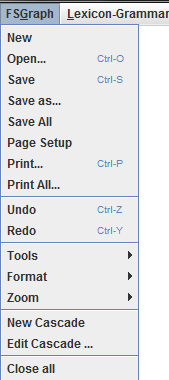
\includegraphics[width=4cm]{resources/img/fig13-08.png}
 \caption{Menu "FSGraph" d'Unitex et sous-menu "New Cascade" et "\textit{Edit cascade...}"}
 \label{fig13-08}
\end{figure}

Le répertoire de la langue courante contient un sous-répertoire nommé CasSys dans lequel se trouvent
les fichiers de configuration d'une cascade. Ce sont des fichiers textes avec l'extension \textit{.csc} (ex: ma cascade.csc)

\subsection{Edition de la liste des transducteurs}
\label{subsec:editlistTrans}

La fenêtre de configuration de CasSys (\ref{fig13-03}) comporte trois parties :

\begin{figure}[!htb]
  \centering
  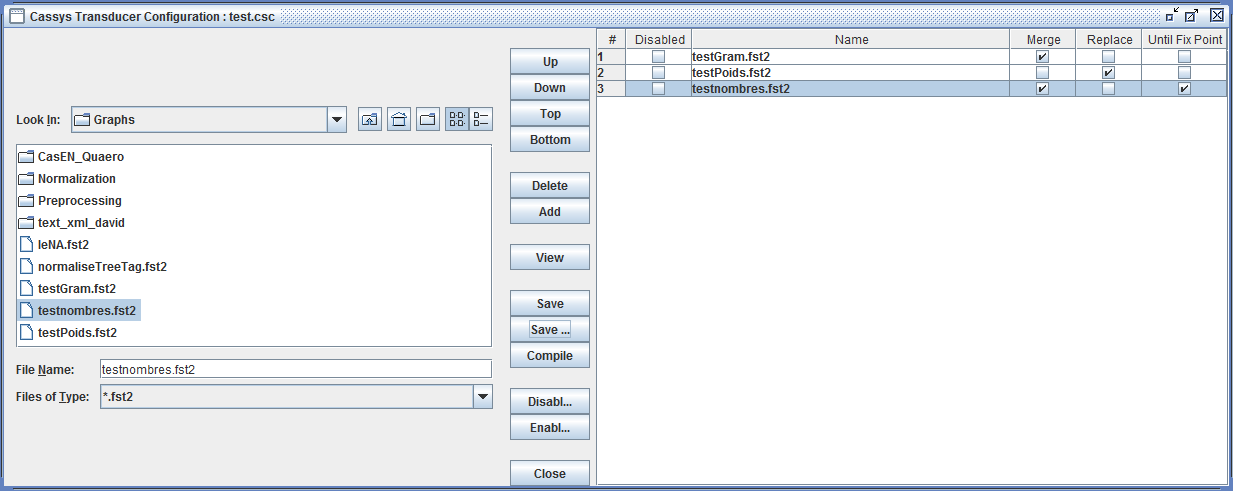
\includegraphics[width=16cm]{resources/img/fig13-03.png}
  \caption{Fenêtre de configuration de CasSys avec à droite la liste des transducteurs}
  \label{fig13-03}
\end{figure}

\begin{enumerate}
	\item Un \textit{gestionnaire de fichier} à gauche du cadre permet de choisir les transducteurs à mettre dans la cascade.
	Le gestionnaire n'affiche que les fichiers fst2 (tous les graphes que vous souhaitez mettre dans la liste doivent être compilés au format fst2).
	
	Pour éditer la cascade, choisissez les graphes à gauche et mettez les à droite à l'aide d'un glisser-déposer.
\item Le \textit{tableau} de droite affiche la cascade: la liste ordonnée des transducteurs et les options sélectionnées pour chaque graphe.
		Le tableau est évidemment vide pour une nouvelle cascade.
		 
		Les colonnes du tableau (Figure \ref{fig13-09}) donne le numéro de chaque graphe et permettent de choisir leur comportement.
	\begin{itemize}
	\item \textbf{\#} : Numéro du graphe/transducteur dans la cascade pour chaque graphe; le fichier fst2 est numéroté.
	\item \textbf{Disabled} : Pour désélectionner le graphe courant. \textit{Disabled} siginifie: "\textit{non appliqué dans la cascade}".
		Les graphes non sélectionnés apparaissent sans numéro, en grisé et barré.
	\item \textbf{Name} : Le nom du graphe (avec l'extension \emph{fst2}). Si vous laissez la souris sur le nom du graphe,
		une info-bulle apparaît avec le chemin complet du graphe.
		Les graphes dont le fichier source n'est pas trouvé apparaissent en italique et en rouge.

	\item \textbf{Merge}: Si le transducer doit être appliqué en mode merge.
	\item \textbf{Replace}: Si le transducer doit être appliqué en mode replace.
	\item \textbf{Until fix point}: Si le transducteur doit être appliqué une fois ou plusieurs fois
		jusqu'à ce que le texte soit inchangé c'est à dire qu'un point fixe est atteint (voir \ref{sub:AppWhiCon}).
	\end{itemize}
	
	 \item Au centre se trouvent les boutons décrits ci-dessous:
		\begin{itemize}
		\item \textit{"Up"/"Down"/"Top"/"Bottom"} sont utilisés pour modifier l'ordre
		des transducteurs dans la liste (ils déplacent le transducteur sélectionné); 
		\textit{"Up"} et \textit{"Down"} déplacent le transducteur sélectionné d'une ligne vers le haut ou
			vers le bas, \textit{"Top"} et \textit{"Bottom"} le positonnent au début ou à la fin de la liste.
		\item \textit{"Delete"} permet de supprimer le transducteur sélectionné de
		la liste des transducteurs. 
		\item \textit{"Add"} ajoute un transducteur (précédemment sélectionné) dans la liste.
			Il remplace le gisser-déposer préalablement décrit.
		\item \textit{"View"} ouvre le graphe sélectionné aussi bien dans l'explorateur
		de fichiers que dans la liste de transducteurs. Il est très utile d'avoir un accès
		rapide à n'importe quel transducteur aussi bien pour y jeter un coup d'œil que pour
		le modifier.
		\item \textit{"Save"} et \textit{"Save as"} permettent d'enregistrer la
		liste des transducteurs. Par défaut, les listes des transducteurs sont placées dans
		le répertoire CasSys de la langue courante  (par exemple French/Cassys).
		\item \textit{"Compile"} recompile tous les graphes de la cascade.	
		\item \textit{"Disable all"} pour désélectionner tous les graphes de la cascade.	
		\item \textit{"Enable all"} pour sélectionner tous les graphes de la cascade.	
		\item \textit{"Close"} ferme la fenêtre courante.
		\end{itemize}
\end{enumerate}


\begin{figure}[!htb]
  \centering
  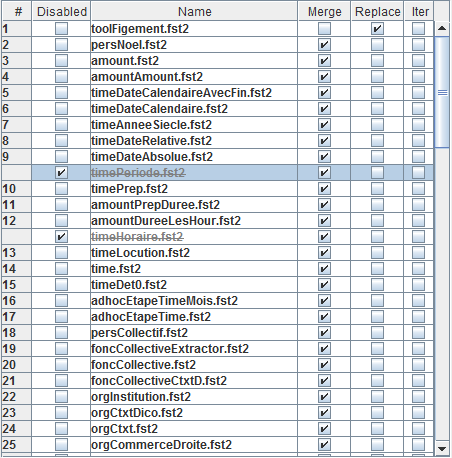
\includegraphics[width=7cm]{resources/img/fig13-09.png}
  \caption{La table/liste de transducteurs}
  \label{fig13-09}
\end{figure}

	

\subsection{Application d'une cascade}
\label{subsec:launchCascade}

Dans le menu "Text", sélectionner le sous-menu "\textit{Apply CasSys cascade...}" (Figure \ref{fig13-01}) pour ouvrir la fenêtre CasSys.
Ce sous-menu "\textit{Apply CasSys cascade...}" n'est actif que si un texte a été préalablement ouvert.

\begin{figure}[!htb]
 \centering
 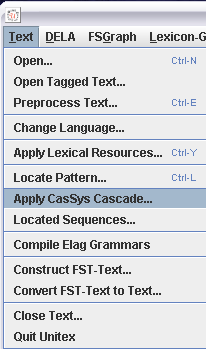
\includegraphics[width=5cm]{resources/img/fig13-01.png}
 \caption{Menu "Text" d'Unitex et sous-menu "Apply CasSys Cascade"}
 \label{fig13-01}
\end{figure}

La fenêtre CasSys (\ref{fig13-02}) affiche le contenu du répertoire CasSys de la langue courante. Elle
permet de choisir le fichier contenant la liste de transducteurs à appliquer au texte. Une fois que cette liste
est choisie, vous pouvez cliquer sur le bouton "Launch" pour appliquer la cascade.

\begin{figure}[!htb]
  \centering
  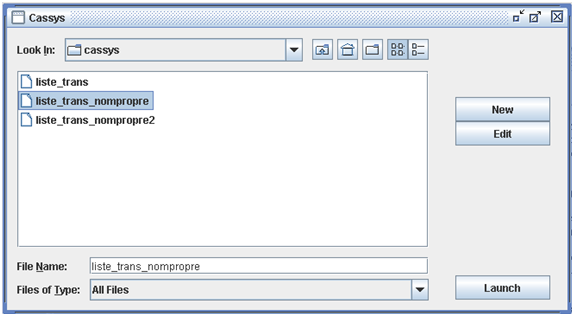
\includegraphics[width=10cm]{resources/img/fig13-02.png}
  \caption{Fenêtre de lancement de la cascade de transducteurs}
  \label{fig13-02}
\end{figure}

N'importe quel dictionnaire du mode morphologique déclaré dans vos préférences est utlisable dans vos
graphes.
Les  préférences peuvent être modifiées à partir du menu "Info" (Info -->
Preferences --> morphological-mode dictionaries).

\subsection{Partage d'un fichier liste de transducteurs en cascade}
\label{subsec:shareCascade}

Afin de faciliter le travail collaboratif avec CasSys, une fonctionnalité d'export/import est
fournie à l'aide d'un fichier liste de transducteurs. Cette possibilité est offerte par le menu
"\textit{Text / Apply CasSys cascade...}" (Figure \ref{fig13-02}).

Pour partager un fichier liste de cascade, les points suivants doivent être remplis:
\begin{enumerate}
\item \textbf{Export :} Choisissez un fichier cascade et cliquez sur le bouton "export".
	(Un fichier partageable est créé dans le répertoire \texttt{/Cassys/Share})
\item Envoyez le fichier partagé à vos collègues
\item \textbf{Import :} Choisissez un fichier  et cliquez sur le bouton "import".
	(Un fichier prêt à être utilisé est créé dans le répertoire \texttt{/Cassys})
\end{enumerate}

%%%%%%%%%%%%%%%%%%%%%%%%%%%%%%%%%%%%%%%%%%%%%%%%%%%%%%%
\section{CasSys en détail}

Dans cette section nous présentons une description détaillée du fonctionnement de CasSys.

\subsection{Type de graphe utilisé}
\label{graphs-for-cassys}

CasSys utilise la version compilée des graphes (format \verb+.fst2+). CasSys gère les grammaires locales
(section~\ref{syntactic-graphs}) présentées dans le chapitre \ref{chap-advanced-grammars}.
Les grammaires utilisées dans une cascade suivent les mêmes règles que les grammaires habituellement
utilisées dans Unitex. Elles peuvent comporter des sous-graphes, utiliser le mode morphologique et les filtres
morphologiques, et faire référence aux informations présentes dans les dictionnaires. 

\bigskip
\noindent CasSys n'est pas compatible avec les fichiers \verb+fst2+ en mode debug (\ref{section-debug-mode}).
Quand on applique un graphe en mode debug avec le menu \verb+Text>Locate Pattern+, le système
compile le graphe dans un format spécial de mode debug. Pour obtenir un fichier au format \verb+fst2+ normal,
recompilez le graphe, soit avec le menu \verb+FSGraph+, soit en ligne de commande, soit en décochant le mode
debug avant d'appliquer le graphe avec \verb+Locate Pattern+.

\subsection{Application itérative}
\label{sub:AppWhiCon}

Cassys peut appliquer un graphe sur un texte de manière itérative tant que de nouvelles concordances sont obtenues.
Ce comportement est sélectionné ou non pour chaque graphe selon que la case \verb+Until fix point+ est cochée ou non. Cette section présente le comportement de cette option\\

Considérons par exemple le graphe \ref{fig:AB->A} qui reconnait \emph{AB} et le remplace par \emph{A}.\\

\begin{figure}[!htbp]
  \centering
  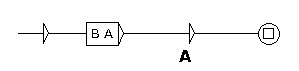
\includegraphics[width=6cm]{resources/img/AB_to_A.png}
  \caption{Transducteur qui modifie BA en A}
  \label{fig:AB->A}
\end{figure}

Considérons le texte \emph{B B B A A A}. L'application du graphe \ref{fig:AB->A} sur ce texte avec \emph{Until fix point}  donne :\\

\begin{tabular}{|l|cccccc|r|}
\hline
initial text  &B&B&B&A&A&A&\\
\hline
itération 1 & &B&B&A&A&A& 1 match\\
itération 2 & & &B&A&A&A& 1 match\\
itération 3 & & & &A&A&A& 1 match\\
itération 4 & & & &A&A&A& 0 match\\
\hline
\end{tabular}

\bigskip
Durant les trois premières itérations, une concordance est obtenue, le graphe
est alors appliqué à nouveau au texte résultant. A la quatrième itération, aucune
concordance n'est trouvée, le graphe n'est donc plus réappliqué.

\bigskip
\large{\textbf{Attention :}} Prendre garde à la possibilité de blocage en utilisant cette 
option. Par exemple, un transducteur qui reconnaît \emph{A} et le remplace par
\emph{A} causerait un blocage s'il était appliqué sur le texte de l'exemple.

\begin{comment}
\subsection{Un texte au format de type XML avec étiquettes lexicales}

En sortie, le format avec étiquettes lexicales est transformé en un format de type XML.
Ce changement est fait dans le but de proposer un texte plus manipulable  à l'utilisateur final.

A partir de ce format, il est plus facile d'obtenir une sortie adaptable à tous.\\

Plus précisement, les étiquettes lexicales :\\
\begin{tabular}{c}
\texttt{
\{forme.lemme,code1+code2:flex1:flex2\}}
\end{tabular}\\

La sortie CaSsys de type XML a le format suivant :\\
\begin{tabular}{ll}
\texttt{<csc>}&\\
	&\texttt{<form>forme</form>}\\
	&\texttt{<lem>lemme</lem>}\\
	&\texttt{<code>code1</code>}\\
	&\texttt{<code>code2</code>}\\
	&\texttt{<inflect>flex1</inflect>}\\
	&\texttt{<inflect>flex2</inflect>}\\
\texttt{</csc>}&\\
\end{tabular}
\end{comment}


\subsection{Règles utilisées dans une cascade}

Dans une cascade, chaque graphe observe les règles utilisées dans Unitex:
\begin{itemize}
	\item Insertion à gauche des motifs reconnus : en mode "merge", la sortie est insérée à
	gauche de la séquence reconnue.
	\item	Priorité au motif le plus à gauche : lors de l'application d'une grammaire locale,
	les occurrences qui se chevauchent sont toutes indexées. 
	Durant la construction de la concordance, toutes ces occurrences sont présentes, mais comme CasSys
	modifie le texte après application de chaque 
	graphe de la cascade, il est nécessaire de choisir parmi ces occurrences celle à prendre en
	compte. La priorité est donnée à la séquence la plus à gauche.
	\item Priorité au plus long motif: dans CasSys, lors de l'application d'un graphe, c'est la
	séquence la plus longue qui est conservée.
	\item	Limitation du nombre d'occurrences recherchées: dans CasSys, ce nombre n'est pas
	limité : une telle limitation n'a aucun sens dans CasSys. Toutes les occurrences sont
	toujours indexées dans le texte.
\end{itemize}

\subsection{Marquage de motifs dans CasSys}

La sortie des transducteurs peut être utilisée pour insérer des informations dans les textes, en
particulier pour marquer les motifs reconnus: il est possible d'utiliser toute sorte de marques, 
( ), [], "", etc. ou des balises xml comme <xxx> </xxx>, mais CasSys propose une manière
particulière d'annoter les motifs reconnus, offrant certaines possibilités que nous présentons
maintenant.  

\bigskip
\noindent Unitex découpe les textes en tokens de différentes sortes comme le marqueur de fin de
phrase {S}; le marqueur {STOP}, des séquences de lettres contiguës, des étiquettes lexicales
{aujourd'hui,.ADV}, etc. Les étiquettes lexicales sont utilisées dans CasSys de manière
particulière. Une étiquette lexicale (entre accolades) est habituellement utilisée pour éviter les
ambiguïtés (voir les explications à la section \ref{tokenization} et à la section
\ref{section-displaying-sentence-automata}). 
Par exemple, dans un texte, si vous avez le token \emph{\{curly brackets,.N\}}, ni "curly" ni
"brackets" ne seront reconnus, mais seulement la séquence toute entière
"curly brackets". Une étiquette lexicale peut contenir une information lexicale complexe comme
\emph{N+Pers+Hum:fs}.
Dans un graphe, il est possible de chercher un token en utilisant l'information contenue dans un
masque lexical : par exemple, on peut écrire \emph{<.N>} pour chercher 
un nom, \emph{<.Pers+Hum>} pour un être humain ou \emph{<.Pers>}. Ces masques lexicaux sont décrits
dans le chapitre "Recherche d'expressions rationnelles" section
\ref{section-special-symbols}.
 
\bigskip
\noindent Dans CasSys, nous utilisons la marque lexicale de manière particulière. Une cascade de
transducteurs est intéressante pour localiser un îlot de certitude. Il est nécessaire pour ce type
de système d'éviter que des motifs précédemment reconnus soient ambigus avec ceux reconnus par les
graphes suivants. Pour éviter cela, on étiquette les motifs reconnus par les graphes sous la forme
\emph{\{} et \emph{,.tag1+tag2+tagn\}} (où \emph{tag1, tag2, etc.} sont vos propres étiquettes).

\bigskip
\noindent Pour expliciter ce comportement, voici un exemple très simple. Le texte sur lequel nous
travaillons est :

\emph{bac a b c cc a b b ba ab a b bca a b c abaabc}.

\bigskip
\noindent Le graphe grfAB (\ref{fig13-05}) reconnaît la séquence \emph{ab} dans le texte et lui
ajoute l'étiquette lexicale \{a b,.AB\}. Ce graphe appliqué en mode MERGE ajoute \emph{\{ } et
 \emph{,.AB\}} dans le texte.

\begin{figure}[!htb]
  \centering
  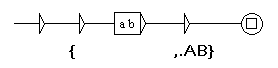
\includegraphics[width=6cm]{resources/img/fig13-05.png}
  \caption{Le graphe grfAB}
  \label{fig13-05}
\end{figure}

\bigskip
\noindent Le texte résultant est : \emph{bac \{a b,.AB\} c cc \{a b,.AB\} b ba ab \{a b,.AB\} bca
\{a b,.AB\} c abaabc}.

\bigskip
\noindent Maintenant le motif \emph{a b} est étiqueté \emph{AB}. La partie (a ou b seul) de ce
motif ne peut pas l'être à cause de l'étiquetage de \emph{a b}.

\bigskip
\noindent Après ce graphe, la cascade applique un autre graphe nommé "tagAB" (\ref{fig13-06})
contenant le masque lexical <AB>. Il reconnait toutes les séquences lexicalement étiquetées par le
graphe précédent.

\begin{figure}[!htb]
  \centering
  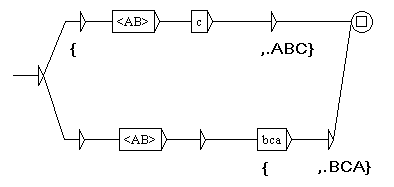
\includegraphics[width=10cm]{resources/img/fig13-06.png}
  \caption{Le graphe tagAB}
  \label{fig13-06}
\end{figure}

\bigskip
\noindent Le texte résultant est : \emph{bac \{\{a b,.AB\} c,.ABC\} cc \{a b,.AB\} b ba ab \{a
b,.AB\} \{bca,.BCA\} \{\{a b,.AB\} c,.ABC\} abaabc}.


\bigskip
\noindent La concordance affichée par Unitex devrait ressembler à celle de la figure
(\ref{fig13-07}). Pour des raisons liées à la programmation (les ambiguïtés entre les
	caractères entre accolades des étiquettes lexicales), nous n'avons d'autres options que de
placer des  $\backslash$ avant chaque caractère ambigu; c'est pourquoi ces symboles sont précédés de
$\backslash$ dans la concordance pour éviter des problèmes avec Unitex.

\begin{figure}[!htb]
  \centering
  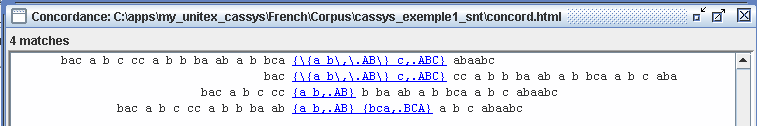
\includegraphics[width=15cm]{resources/img/fig13-07.png}
  \caption{La concordance issue l'application de la cascade}
  \label{fig13-07}
\end{figure}



\section{Les résultats d'une cascade}

\subsection{Affichage des résultats de la cascade}
\label{subsec:resultsCascade}

Le résultat de l'application d'une cascade est un fichier d'index (\textit{concord.ind}), comme c'est le cas
lors d'une recherche de motif avec \textit{"Locate pattern"}. Ce fichier d'index contient toutes les séquences
reconnues conformément aux règles fixées dans Unitex.

\bigskip
\noindent Pour afficher une concordance, il suffit de cliquer sur le bouton "Build concordance"
(comme décrit au chapitre \ref{chap-advanced-grammars}) dans la menu "Text / Located sequences".
La figure \ref{fig13-04} présente un échantillon de concordance d'une cascade qui reconnaît les entités
nommées.


\begin{figure}[!htb]
  \centering
  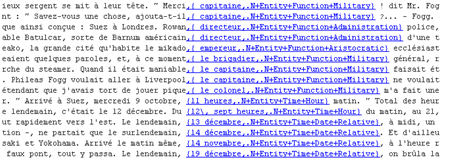
\includegraphics[width=14cm]{resources/img/fig13-04.png}
  \caption{Concordance de CasSys dans Unitex}
  \label{fig13-04}
\end{figure}

\subsection{Les différents fichiers résultats d'une cascade}

CasSys conserve tous les textes créés par chaque graphe  de la cascade. Ceci peut être
utile  pour des tests, le débugage ou la vérification de différents résultats de la cascade. Il est
alors possible de corriger les erreurs selon l'ordre d'application des graphes ou de trouver des
erreurs dans leur écriture. Il est pratique d'ajouter dans la sortie d'un transducteur le nom de ce
dernier, afin de voir dans le résultat final quel motif a été reconnu par quel graphe.

Si l'on applique une cascade au texte exemple.txt, deux répertoires sont créés:
\verb+exemple_snt+ et \verb+exemple_csc+.
Les fichiers créés dans \verb+exemple_csc+ sont les résultats obtenus par
chaque graphe. Ces fichiers sont intitulés selon le numéro du graphe qui les a produit. Par exemple, si le
troisième graphe reconnaît un motif, les résultats de l'application de ce graphe seront stockés dans le 
répertoire  \verb+exemple_3+\newline\verb+_0_snt+ le fichier \verb+exemple_3_0.snt+ contiendra le texte modifié.

\subsection{Un texte au format de type XML pour les étiquettes lexicales}

En sortie, le résultat est fourni sous deux formes~: le texte résultant directement de l'application des transducteurs, et un format de type XML dans lequel les étiquettes lexicales ont été transformées en XML.
Ce changement est fait dans le but de proposer un texte plus manipulable  à l'utilisateur final.
A partir de ce format, il est possible d'utiliser l'un des nombreux outils de traitement du XML.
Il est également facile d'appliquer des transducteurs supplémentaires afin d'obtenir la sortie souhaitée.
Le texte résultant directement des transducteurs est sauvegardé dans le fichier  \verb+exemple_csc.raw+, et la version  XML-isée est dans le fichier \verb+exemple_csc.txt+.

Plus précisement, les étiquettes lexicales sont dans le format suivant~:\\
\begin{tabular}{c}
\texttt{
\{forme.lemme,code1+code2:flex1:flex2\}}
\end{tabular}\\
La sortie de type XML correspondante a le format suivant~:\\
\begin{tabular}{ll}
\texttt{<csc>}&\\
	&\texttt{<form>forme</form>}\\
	&\texttt{<lem>lemme</lem>}\\
	&\texttt{<code>code1</code>}\\
	&\texttt{<code>code2</code>}\\
	&\texttt{<inflect>flex1</inflect>}\\
	&\texttt{<inflect>flex2</inflect>}\\
\texttt{</csc>}&\\
\end{tabular}

La DTD de notre format est la suivante~:

\begin{tabular}{l}
\texttt{<?xml version="1.0" encoding="ISO-8859-1"?>}\\
\texttt{<!ELEMENT text (\#PCDATA|csc)*>}\\
\texttt{<!ELEMENT csc (form,lem?,code*,inflect*) >}\\
\texttt{<!ELEMENT form (\#PCDATA|csc)*>}\\
\texttt{<!ELEMENT lem (\#PCDATA)>}\\
\texttt{<!ELEMENT code (\#PCDATA)>}\\
\texttt{<!ELEMENT inflect (\#PCDATA)>}\\
\end{tabular}



